\documentclass[11pt,oneside]{article}
\usepackage[a4paper,margin=26mm,headheight=15pt]{geometry}
\usepackage[T1]{fontenc}
\usepackage[utf8]{inputenc}
\usepackage{lmodern,microtype}
\usepackage{amsmath,amssymb,amsthm,mathtools,bm}
\usepackage{booktabs,longtable,tabularx,array}
\usepackage{graphicx,xcolor,fancyhdr,enumitem,listings,xurl}
\usepackage[colorlinks=true,linkcolor=blue!45!black,citecolor=blue!45!black,urlcolor=blue!45!black]{hyperref}
\hypersetup{pdftitle={Thue--Morse Beyond the Atlas: Boundary Defects, Nonlinear Prouhet Geometry, and Flat Automatic q-Products},pdfauthor={Research article prepared with ChatGPT},pdfsubject={Exact finite correlation formulas, hypergraph covering identities, and an all-order Lambert-W saddle expansion}}
\numberwithin{equation}{section}
\newtheorem{theorem}{Theorem}[section]
\newtheorem{lemma}[theorem]{Lemma}
\newtheorem{proposition}[theorem]{Proposition}
\newtheorem{corollary}[theorem]{Corollary}
\theoremstyle{definition}
\newtheorem{definition}[theorem]{Definition}
\newtheorem{example}[theorem]{Example}
\newtheorem{question}[theorem]{Research question}
\theoremstyle{remark}
\newtheorem{remark}[theorem]{Remark}
\newcommand{\eps}{\varepsilon}
\newcommand{\NN}{\mathbb N}
\newcommand{\ZZ}{\mathbb Z}
\newcommand{\RR}{\mathbb R}
\newcommand{\CC}{\mathbb C}
\newcommand{\HH}{\mathcal H}
\newcommand{\CCov}{\mathcal C}
\newcommand{\MM}{\mathcal M}
\newcommand{\dd}{\,\mathrm d}
\newcommand{\e}{\mathrm e}
\newcommand{\ii}{\mathrm i}
\DeclareMathOperator{\Haf}{Haf}
\DeclareMathOperator{\supp}{supp}
\DeclareMathOperator{\ord}{ord}
\newcommand{\bits}{\{0,1\}}
\newcommand{\coef}[2]{[#1^{#2}]}
\setlength{\emergencystretch}{3em}
\allowdisplaybreaks[2]
\setlist{itemsep=3pt,topsep=5pt}
\pagestyle{fancy}
\fancyhf{}
\fancyhead[L]{\small Thue--Morse beyond the atlas}
\fancyhead[R]{\small Research article}
\fancyfoot[C]{\thepage}
\renewcommand{\headrulewidth}{0.3pt}
\lstset{basicstyle=\ttfamily\footnotesize,breaklines=true,columns=fullflexible,frame=single,showstringspaces=false}

\begin{document}
\begin{titlepage}
\centering
\vspace*{16mm}
{\large A companion research article to the ProveIt Thue--Morse atlas\par}
\vspace{12mm}
{\LARGE\bfseries Thue--Morse Beyond the Atlas\par}
\vspace{6mm}
{\Large Boundary Defects, Nonlinear Prouhet Geometry,\\[3mm]
and Flat Automatic \(q\)-Products\par}
\vspace{12mm}
{\large Three derived research directions, with proofs and reproducible checks\par}
\vspace{7mm}
{4 September 2026\par}
\vspace{11mm}
\begin{minipage}{0.91\textwidth}
\begin{abstract}
The signed Thue--Morse sequence connects binary carries, cancellation of moments,
and products across geometric scales. We develop three refinements of these
connections. First, a single finite boundary functional gives the exact dyadic
correlation defect at every order: even correlations have an alternating defect,
whereas odd correlations become an explicit telescoping difference after dyadic
blocking. The same functional yields formulas for arbitrary numbers of complete
blocks, without a recursive correlation hierarchy. Second, we transport the
Thue--Morse signs to nonlinear Boolean-cube coordinates. An exact covering-family
identity identifies the cancellation order with a hypergraph covering number
for positive weights. Quadratic deformations lead to hafnians, explicit path
formulas, and a monomer--dimer crossover polynomial. Third, we study the geometric
product
\(\Phi_q(z)=\prod_{j\ge0}(1-zq^j)^{\eps_j}\).
It is flat to every algebraic order as \(q\to1^-\), but its logarithm has a
nontrivial all-order saddle expansion with an explicit Lambert-\(W\) parameter
and a smooth periodic amplitude. The amplitude is expressed exactly through a
dyadic uniform-convolution Laplace product, making the Fabius connection precise. A joint endpoint scaling recovers
classical paired products with every algebraic correction absent.
The article distinguishes classical ingredients from the present derived
formulas. Historical priority is not asserted: these are candidates for new
results relative to the inspected atlas and the targeted literature, rather
than a certified exhaustive novelty claim.
\end{abstract}
\end{minipage}
\vfill
\begin{minipage}{0.91\textwidth}
\small
\textbf{Status.} Self-contained mathematical research draft prepared with
ChatGPT. The main statements have proofs and independent computational checks;
no claim of peer review or Lean formalization is made. The accompanying archive
contains the standalone \LaTeX\ source, PDF, commented verification program,
computed tables, and source-audit notes.
\end{minipage}
\end{titlepage}

\tableofcontents
\clearpage

\section{Scope, sources, and the contribution map}
\label{sec:scope}

\subsection{What is being extended}
The linked \emph{Thue--Morse Atlas and Frontiers} in Vladimir Reshetnikov's
ProveIt repository is the starting point \cite{atlas}. Its product identities,
finite-block calculus, moment formulas, and Fabius--Rvachev connections provide
a substantial foundation. Accordingly, this article does not present the
classical generating product or Prouhet cancellation as discoveries. It uses
them as short, explicitly proved lemmas and develops three more specialized
constructions.

The correlation literature is particularly important for avoiding overstatement.
Baake and Coons show how higher-order correlations are controlled by a basic
balanced two-point value, and establish the vanishing of odd-order correlations
\cite{baakecoons}. Our correlation contribution is an explicit
\emph{finite-size boundary formula}, not a claim to have discovered higher-order
correlations or their basic renormalization. Likewise, the nonlinear moment
section uses classical Boolean inclusion--exclusion, and the analytic section
uses a classical saddle-point method. New research can lie in the exact objects
these methods expose, rather than in inventing the methods themselves.

\subsection{The three directions}
\begin{description}[leftmargin=0pt,labelsep=0.7em]
\item[Boundary defects.] For an arbitrary finite tuple of shifts, a signed sum
of at most as many terms as the largest shift determines all finite dyadic
correlation corrections. For even order, the only remaining scale dependence
is \((-1)^m\). For odd order, the sum over the \(q\)-th sufficiently large dyadic
block is a constant multiple of \(\eps_{q+1}-\eps_q\).
\item[Nonlinear Prouhet geometry.] The signs stay fixed, but the point with
binary digits \(b\) is moved to a multilinear polynomial \(x(b)\). The first
surviving moment is governed by covers of the bit positions. Pair interactions
produce perfect matchings and hafnians; weak pair interactions produce a full
matching polynomial.
\item[Flat automatic products.] A Thue--Morse-weighted \(q\)-Pochhammer-type
product tends to one faster than every power of \(-\log q\). Its small deviation
is nevertheless computable: a growing family of terms, centered at an explicit
Lambert-\(W\) saddle, is modulated by an exact log-periodic function.
\end{description}

These three directions share a useful principle: the dyadic structure can often
be isolated into a finite combinatorial quantity or a bounded periodic function.
What remains can then be analyzed without repeatedly expanding the entire
Thue--Morse word.

\subsection{Novelty audit and its limitations}
The source review covered the linked consolidated \LaTeX\ article, its visible
section structure and relevant passages, and targeted external searches. The
reference list records primary mathematical sources. A complete recursive,
commit-pinned checkout of every document in the repository was not obtained;
therefore no claim of exhaustive nonduplication is justified. The consulted
\texttt{main} source is mutable, and the access date is 4 September 2026.

The classical survey by Allouche and Shallit \cite{ubiquitous} supplies the
background context. Generalized Prouhet constructions are discussed by Bolker,
Offner, Richman, and Zara \cite{bolker}. The 2026 preprint of Cloitre \cite{cloitre}
was also screened: its transform of binary words and induced partitions provide
a different direction from the fixed-sign nonlinear coordinates considered
here. Products weighted by Thue--Morse signs already form an established subject
\cite{ars,li}; the distinction here is the geometric argument \(q^j\) and its
singular limit. The harmonic-sum viewpoint of Flajolet, Gourdon, and Dumas
\cite{fgd} provides analytic context.

The results below are thus presented as \emph{proved derived refinements and
novelty candidates}, with the exact formulas available for further literature
comparison. They should not be advertised as the first results of their kind
without an additional specialist priority review.

\section{Binary and analytic preliminaries}
\label{sec:prelim}

We use zero-based indexing. For \(n\ge0\), let \(s_2(n)\) be the number of ones
in its binary expansion and define
\begin{equation}
 \eps_n=(-1)^{s_2(n)}.
 \label{eq:eps}
\end{equation}
Thus the first sixteen signs are
\[
 1,-1,-1,1,-1,1,1,-1,-1,1,1,-1,1,-1,-1,1.
\]
Empty products are one. A repeated shift in a correlation is permitted; its
multiplicity is part of the definition.

\begin{lemma}[Block and reflection identities]
For \(N=2^m\), \(q\ge0\), and \(0\le r<N\),
\begin{equation}
 \eps_{qN+r}=\eps_q\eps_r,
 \qquad
 \eps_{N-1-r}=(-1)^m\eps_r.
 \label{eq:blocks}
\end{equation}
If \(m\ge1\), then, with the index interpreted modulo \(N\),
\begin{equation}
 \eps_{(r+N/2)\bmod N}=-\eps_r.
 \label{eq:halfperiod}
\end{equation}
\end{lemma}
\begin{proof}
The binary digits of \(qN\) and \(r\) occupy disjoint positions, so their digit
sums add. Subtraction from \(N-1\) complements exactly \(m\) digits, proving the
second formula. Adding \(N/2\) modulo \(N\) toggles the highest of those digits
and leaves the others unchanged, proving the third.
\end{proof}

\begin{lemma}[The generating product]
For \(|z|<1\),
\begin{equation}
 E(z):=\sum_{n\ge0}\eps_nz^n
       =\prod_{j\ge0}(1-z^{2^j}),
 \qquad E(z)=(1-z)E(z^2).
 \label{eq:E}
\end{equation}
The product converges locally uniformly in the unit disk.
\end{lemma}
\begin{proof}
In the finite product through \(j=m-1\), choosing the factor \(-z^{2^j}\)
exactly for the one-bits of \(n<2^m\) gives the coefficient \(\eps_n\). Hence
\(\prod_{j<m}(1-z^{2^j})=\sum_{n<2^m}\eps_nz^n\). For \(|z|\le\rho<1\),
\(\sum_j\rho^{2^j}<\infty\), so the product converges uniformly there. Passing
to the limit gives the identity. Removing its first factor gives the functional
equation.
\end{proof}

\subsection{An exact adjacent-correlation sum}
The following elementary identity will replace an infinite correlation
recursion by a finite binary-digit expression.

\begin{definition}
For an integer \(Q=\sum_{j\ge0}b_j2^j\ge0\), define the alternating digit sum
\begin{equation}
 \sigma(Q)=\sum_{j\ge0}(-1)^jb_j.
 \label{eq:sigma}
\end{equation}
In particular, \(\sigma(0)=0\) and \(\sigma(2^k)=(-1)^k\).
\end{definition}

\begin{lemma}[Adjacent correlation at every endpoint]
For every \(Q\ge0\),
\begin{equation}
 C(Q):=\sum_{q=0}^{Q-1}\eps_q\eps_{q+1}
       =-\frac Q3-\frac23\sigma(Q).
 \label{eq:C}
\end{equation}
Consequently \(C(Q)/Q\to-1/3\) as \(Q\to\infty\).
\end{lemma}
\begin{proof}
Write \(c(q)=\eps_q\eps_{q+1}\). The binary recursion gives
\(c(2q)=-1\) and \(c(2q+1)=-c(q)\). Therefore
\[
 C(2Q)=-Q-C(Q),\qquad C(2Q+1)=-Q-C(Q)-1.
\]
On the other hand,
\(\sigma(2Q)=-\sigma(Q)\) and
\(\sigma(2Q+1)=1-\sigma(Q)\). Substitution shows that the proposed right-hand
side satisfies the same recurrences and agrees at zero; induction proves the
formula. The number of nonzero summands in \(\sigma(Q)\) is at most the binary
length of \(Q\), which is \(O(\log(Q+1))\). Division by \(Q\) proves the limit.
\end{proof}

\section{Exact boundary defects for correlations of every order}
\label{sec:correlations}

\subsection{The finite boundary functional}
Fix a tuple
\[
 \bm h=(h_1,\ldots,h_p),\qquad p\ge1,\qquad
 0=\min_i h_i,\qquad H=\max_i h_i.
\]
For \(N=2^m>H\), define the noncyclic and cyclic sums
\begin{align}
 S_m(\bm h)&=\sum_{n=0}^{N-1}\prod_{i=1}^p\eps_{n+h_i},
 \label{eq:Sm}\\
 R_m(\bm h)&=\sum_{n=0}^{N-1}\prod_{i=1}^p
                 \eps_{(n+h_i)\bmod N}.
 \label{eq:Rm}
\end{align}
The noncyclic sum uses the infinite sequence even when a shifted index exits
the first block. The distinction between these two conventions is essential.

For each \(1\le t\le H\), set
\begin{align}
 b_t&=\#\{i:h_i\ge t\},\\
 G_t(\bm h)&=
 \prod_{h_i<t}\eps_{t-h_i-1}
 \prod_{h_i\ge t}\eps_{h_i-t}.
 \label{eq:Gt}
\end{align}
Define the \emph{boundary functional}
\begin{equation}
 D(\bm h)=\sum_{\substack{1\le t\le H\\b_t\text{ odd}}}G_t(\bm h).
 \label{eq:defect}
\end{equation}
It is an integer and satisfies \(|D(\bm h)|\le H\). All its sign indices lie
between zero and \(H-1\), so it is independent of the dyadic level \(m\).

\begin{theorem}[One boundary functional, all dyadic levels]
\label{thm:boundary}
Suppose \(m\ge1\) and \(N=2^m>H\).

If \(p\) is even, the correlation mean
\begin{equation}
 \eta(\bm h)=\lim_{X\to\infty}\frac1X
       \sum_{n=0}^{X-1}\prod_i\eps_{n+h_i}
 \label{eq:eta}
\end{equation}
exists, and
\begin{align}
 S_m(\bm h)&=N\eta(\bm h)-\frac23(-1)^mD(\bm h),
 \label{eq:evenS}\\
 R_m(\bm h)&=N\eta(\bm h)+\frac43(-1)^mD(\bm h).
 \label{eq:evenR}
\end{align}
If \(p\) is odd, the same mean exists and equals zero, while
\begin{equation}
 S_m(\bm h)=-2D(\bm h),\qquad R_m(\bm h)=0.
 \label{eq:oddS}
\end{equation}
\end{theorem}

\begin{proof}
Write an index as \(n=qN+r\), with \(0\le r<N\), and let
\[
 \chi_i(r)=\boldsymbol 1_{\{r+h_i\ge N\}},\quad
 b(r)=\sum_i\chi_i(r),\quad
 g(r)=\prod_i\eps_{(r+h_i)\bmod N}.
\]
Because \(h_i<N\), each shifted index crosses at most one block boundary.
The block identity \eqref{eq:blocks} gives the exact factorization
\begin{equation}
 \prod_i\eps_{qN+r+h_i}
   =g(r)\eps_q^{p-b(r)}\eps_{q+1}^{b(r)}.
 \label{eq:blockfactor}
\end{equation}
Separate the local sums according to the parity of the crossing number:
\[
 U_m=\sum_{b(r)\text{ even}}g(r),\qquad
 V_m=\sum_{b(r)\text{ odd}}g(r).
\]
Thus \(R_m=U_m+V_m\).

We first compute \(V_m\). An odd crossing number can occur only at
\(r=N-t\), \(1\le t\le H\). A noncrossing index then has the form
\(N-(t-h_i)\); reflection in \eqref{eq:blocks} turns its sign into
\((-1)^m\eps_{t-h_i-1}\). A crossing index has the local value \(h_i-t\).
There are \(p-b_t\) noncrossing indices. On the terms selected for \(V_m\),
\(b_t\) is odd, so
\begin{equation}
 V_m=
 \begin{cases}
  (-1)^mD(\bm h),&p\text{ even},\\
  D(\bm h),&p\text{ odd}.
 \end{cases}
 \label{eq:Vm}
\end{equation}

Suppose now that \(p\) is even. Summing \eqref{eq:blockfactor} over one block
produces
\begin{equation}
 \sum_{r=0}^{N-1}\prod_i\eps_{qN+r+h_i}
       =U_m+V_m\eps_q\eps_{q+1}.
 \label{eq:evenblock}
\end{equation}
Over \(Q\) complete blocks, division by \(QN\) and use of \eqref{eq:C} give
\(\eta=(U_m-V_m/3)/N\). An arbitrary endpoint leaves fewer than \(N\) terms,
whose contribution to the average tends to zero. This proves existence of the
full limit. At \(q=0\), \(\eps_0\eps_1=-1\), hence \(S_m=U_m-V_m\). Combining
this with \(R_m=U_m+V_m\), the formula for \(\eta\), and \eqref{eq:Vm} proves
\eqref{eq:evenS}--\eqref{eq:evenR}.

If \(p\) is odd, the cyclic sum is zero: shifting every summation index by
\(N/2\) reverses all \(p\) signs by \eqref{eq:halfperiod}. Consequently
\(U_m=-V_m=-D(\bm h)\). Formula \eqref{eq:blockfactor} now gives
\begin{equation}
 \sum_{r=0}^{N-1}\prod_i\eps_{qN+r+h_i}
       =D(\bm h)(\eps_{q+1}-\eps_q).
 \label{eq:oddblock}
\end{equation}
This telescopes over \(q\), so the sum over any number of complete blocks is
bounded by \(2|D|\). A partial final block has fewer than \(N\) terms.
The correlation mean is therefore zero. Taking \(q=0\) proves
\eqref{eq:oddS}.
\end{proof}

\begin{remark}[What is and is not new in this statement]
The means and their renormalization belong to the established correlation
theory \cite{baakecoons}. The refinement emphasized here is the explicit finite
functional \eqref{eq:defect}, its independence of \(m\), and the exact boundary
and telescoping formulas. The proof also shows why the number of correlation
factors does not introduce additional dyadic defect modes: once a block is
longer than every shift, the only coarse signs available are \(\eps_q\) and
\(\eps_{q+1}\).
\end{remark}

\subsection{All block multiples and aligned intervals}
Write
\[
 S_{m,Q}(\bm h)=\sum_{n=0}^{QN-1}\prod_i\eps_{n+h_i},\qquad Q\ge0.
\]

\begin{corollary}[Exact endpoint formulas]
\label{cor:blockmultiples}
Under the assumptions of Theorem~\ref{thm:boundary},
\begin{equation}
 S_{m,Q}(\bm h)=
 \begin{cases}
 QN\eta(\bm h)-\dfrac23(-1)^mD(\bm h)\sigma(Q),&p\text{ even},\\[2mm]
 D(\bm h)(\eps_Q-1),&p\text{ odd}.
 \end{cases}
 \label{eq:allblocks}
\end{equation}
In particular, the sum over the aligned interval \([AN,BN)\) is obtained by
subtracting the same expression at \(Q=A\) from that at \(Q=B\).
\end{corollary}
\begin{proof}
For even \(p\), sum \eqref{eq:evenblock} and use
\(U_m=N\eta+V_m/3\), \eqref{eq:C}, and \eqref{eq:Vm}.
For odd \(p\), telescope \eqref{eq:oddblock}. Interval subtraction is exact.
\end{proof}

Thus finite endpoints are controlled either by the alternating digit sum of
\(Q\) or by its Thue--Morse sign. For a fixed tuple, the odd-order partial sums
are bounded uniformly in the endpoint. Even-order centered partial sums have
an elementary logarithmic bound.

\begin{corollary}[Discrepancy bounds]
For fixed \(\bm h\), let \(X=QN+R\), \(0\le R<N\). If \(p\) is even, then
\begin{equation}
 \left|\sum_{n<X}\prod_i\eps_{n+h_i}-X\eta(\bm h)\right|
 \le \frac23|D(\bm h)|\,|\sigma(Q)|+2N.
 \label{eq:disc-even}
\end{equation}
If \(p\) is odd, then
\begin{equation}
 \left|\sum_{n<X}\prod_i\eps_{n+h_i}\right|
 \le 2|D(\bm h)|+N.
 \label{eq:disc-odd}
\end{equation}
\end{corollary}
\begin{proof}
Apply \eqref{eq:allblocks}. A partial block contains at most \(N\) signs of
absolute value one, and \(|\eta|\le1\), so centering that partial block costs
at most \(2N\). In the odd case no centering is necessary.
\end{proof}

The even bound is \(O_{\bm h}(\log(X+2))\), while the odd bound is
\(O_{\bm h}(1)\). Neither statement is asserted to have an optimal constant.
For shifts growing with \(X\), the explicit dependence on \(H\) and \(N\) must
be retained; a fixed-shift estimate must not be used as a uniform growing-shift
estimate.

\subsection{Two-level extraction and rationality}
\begin{corollary}[Exact extrapolation, not an asymptotic approximation]
If \(p\) is even and \(N=2^m>H\),
\begin{equation}
 \eta(\bm h)=\frac{S_m(\bm h)+S_{m+1}(\bm h)}{3N}
           =\frac{R_m(\bm h)+R_{m+1}(\bm h)}{3N}.
 \label{eq:twolevels}
\end{equation}
Moreover,
\begin{equation}
 \eta(\bm h)\in\frac1{3N}\ZZ,\qquad
 \left|\frac{S_m}N-\eta\right|\le\frac{2H}{3N},\qquad
 \left|\frac{R_m}N-\eta\right|\le\frac{4H}{3N}.
 \label{eq:ratbound}
\end{equation}
\end{corollary}
\begin{proof}
The defects in consecutive dyadic levels have opposite signs and equal
magnitudes. Adding the two exact formulas cancels them, while the main terms
sum to \(3N\eta\). The rationality and inequalities follow from integrality of
\(S_m,D\) and \(|D|\le H\).
\end{proof}

The frequency module with denominators consisting of a factor three and powers
of two is already part of the classical structure \cite{baakecoons}. Here it
is recovered together with an explicit finite extraction formula.

\subsection{Pairs, a convolution coefficient, and examples}
For \(\bm h=(0,h)\), the odd crossing number is one throughout the boundary,
so
\begin{equation}
 D(0,h)=\sum_{j=0}^{h-1}\eps_j\eps_{h-1-j}
       =[z^{h-1}]E(z)^2\qquad(h\ge1).
 \label{eq:pairD}
\end{equation}
This is a useful bridge between a finite correlation defect and the ordinary
generating series.

\begin{proposition}[Binary recursion for the pair defect]
With \(D_h=D(0,h)\), set \(D_0=0\). Then \(D_1=1\), and
\begin{equation}
 D_{2h}=-2D_h,\qquad D_{2h+1}=D_h+D_{h+1}.
 \label{eq:Drec}
\end{equation}
\end{proposition}
\begin{proof}
Write \(a_n=[z^n]E(z)^2\), with \(a_{-1}=0\). Squaring
\(E(z)=(1-z)E(z^2)\) gives
\(a_{2n}=a_n+a_{n-1}\) and \(a_{2n+1}=-2a_n\).
Since \(D_h=a_{h-1}\), the claimed formulas follow, including the boundary
values.
\end{proof}

\begin{table}[htbp]
\centering
\caption{Exact even-order examples. Here \(N=2^m>H\), and cyclic and
noncyclic sums use the conventions in \eqref{eq:Sm}--\eqref{eq:Rm}.}
\label{tab:corr}
\begin{tabular}{@{}lrrrrr@{}}
\toprule
Shifts \(\bm h\)&\(m\)&\(D\)&\(\eta\)&\(S_m\)&\(R_m\)\\
\midrule
\((0,1)\)&1&1&\(-1/3\)&0&\(-2\)\\
\((0,2)\)&2&\(-2\)&\(-1/3\)&0&\(-4\)\\
\((0,3)\)&2&\(-1\)&\(1/3\)&2&0\\
\((0,1,2,3)\)&2&2&\(1/3\)&0&4\\
\((0,1,3,7)\)&3&\(-3\)&0&\(-2\)&4\\
\((0,2,5,9)\)&4&\(-2\)&\(1/6\)&4&0\\
\((0,1,2,4,7,11)\)&4&\(-5\)&\(-1/3\)&\(-2\)&\(-12\)\\
\bottomrule
\end{tabular}
\end{table}

\begin{example}[A zero mean with a persistent dyadic boundary signal]
For \(\bm h=(0,1,3,7)\), Table~\ref{tab:corr} gives \(\eta=0\), \(D=-3\).
For every \(m\ge3\),
\[
 S_m=2(-1)^m,\qquad R_m=-4(-1)^m.
\]
The unnormalized finite signal does not tend to zero even though its normalized
mean does. Cyclic and noncyclic experiments detect different boundary signals.
\end{example}

\begin{example}[An odd-order telescoping observable]
For \(\bm h=(0,1,2)\), \(D=-1\). Every dyadic block of length \(N\ge4\)
satisfies
\[
 \sum_{r=0}^{N-1}\eps_{qN+r}\eps_{qN+r+1}\eps_{qN+r+2}
 =\eps_q-\eps_{q+1}.
\]
Thus the sum up to \(QN\) is exactly \(1-\eps_Q\), taking only the values zero
and two. This is stronger information than vanishing of the limiting mean.
\end{example}

\subsection{A nonrecursive algorithm}
To evaluate an even correlation mean, choose
\(m=\max(1,\lceil\log_2(H+1)\rceil)\). Compute one block sum and the
boundary functional, then use
\[
 \eta(\bm h)=\frac{3S_m(\bm h)+2(-1)^mD(\bm h)}{3\cdot2^m}.
\]
For fixed order \(p\), a direct implementation uses \(O(pH)\) sign evaluations,
up to the harmless factor coming from \(2^m<2(H+1)\). The integer digit-parity
operation makes each sign inexpensive. This is a transparent alternative to
recursively reducing a large family of correlation tuples. It is not a claim
that this direct algorithm beats every specialized recursion.

\section{Nonlinear Prouhet cancellation as a covering problem}
\label{sec:hypergraph}

\subsection{Moving the points while keeping the signs}
The usual Prouhet sum assigns the sign \((-1)^{b_0+\cdots+b_{m-1}}\) to the
point \(\sum_i2^ib_i\). We retain the signs but allow nonlinear coordinates.
Let \(V=\{0,\ldots,m-1\}\), let \(\HH\) be a finite family of nonempty subsets
of \(V\), and put
\begin{equation}
 x(b)=c_0+\sum_{S\in\HH}c_S b_S,
 \qquad b_S=\prod_{i\in S}b_i,
 \qquad b\in\bits^m.
 \label{eq:geometry}
\end{equation}
Terms with zero coefficient can be removed. Every function on the Boolean cube
has a unique multilinear representation, but sparsity of \(\HH\) is what makes
the following description informative.

Define the signed exponential generating function
\begin{equation}
 Z_x(t)=\sum_{b\in\bits^m}(-1)^{|b|}\e^{t x(b)}
       =\sum_{r\ge0}\frac{t^r}{r!}
           \sum_{b\in\bits^m}(-1)^{|b|}x(b)^r.
 \label{eq:Z}
\end{equation}
A subfamily \(\CCov\subseteq\HH\) is a \emph{cover} if
\(\bigcup_{S\in\CCov}S=V\). Let \(\tau(\HH)\) be the minimum number of
members in a cover, and set \(\tau=\infty\) if there is no cover.

\begin{theorem}[Exact covering-family identity]
\label{thm:cover}
For every complex \(t\) and all complex coefficients in \eqref{eq:geometry},
\begin{equation}
 Z_x(t)=(-1)^m\e^{tc_0}
 \sum_{\substack{\CCov\subseteq\HH\\\bigcup_{S\in\CCov}S=V}}
       \prod_{S\in\CCov}(\e^{tc_S}-1).
 \label{eq:cover}
\end{equation}
\end{theorem}
\begin{proof}
On the Boolean cube, \(b_S\) takes only the values zero and one, hence
\[
 \e^{tc_Sb_S}=1+(\e^{tc_S}-1)b_S.
\]
Multiply these identities over \(S\in\HH\). Choosing the nonconstant term
for the subfamily \(\CCov\) contributes
\(\prod_{S\in\CCov}(\e^{tc_S}-1)b_U\), where
\(U=\bigcup_{S\in\CCov}S\); repeated bit factors collapse because
\(b_i^2=b_i\). The signed cube sum of \(b_U\) factors over coordinates. If
any coordinate is missing from \(U\), its factor is \(1-1=0\). If \(U=V\),
only the all-one vertex contributes, and its sign is \((-1)^m\).
Multiplying by \(\e^{tc_0}\) proves \eqref{eq:cover}.
\end{proof}

\begin{corollary}[Cover number and the first surviving moment]
\label{cor:coverorder}
If \(\tau<\infty\), then
\begin{equation}
 \sum_b(-1)^{|b|}x(b)^r=0\quad(0\le r<\tau),
 \label{eq:covervanish}
\end{equation}
and
\begin{equation}
 \sum_b(-1)^{|b|}x(b)^\tau
 =(-1)^m\tau!
  \sum_{\substack{\CCov\text{ cover}\\|\CCov|=\tau}}
       \prod_{S\in\CCov}c_S.
 \label{eq:coverlead}
\end{equation}
If all \(c_S>0\), this is nonzero, so the vanishing order of \(Z_x\) at zero
is exactly \(\tau\). If there is no cover, then \(Z_x\equiv0\).
\end{corollary}
\begin{proof}
Every factor \(\e^{tc_S}-1\) begins with \(tc_S\), so a cover with \(k\)
members contributes first at order \(t^k\). At the minimum order only its
linear terms contribute. The constant-coordinate factor starts with one and
does not affect that coefficient. For positive weights all minimum-cover
contributions have the same sign. If there is no cover, the sum in
\eqref{eq:cover} is empty.
\end{proof}

\begin{remark}[A cancellation caveat]
For negative or complex weights, the minimum-cover sum may vanish. Then
\(\tau\) is a lower bound on the vanishing order, not necessarily its exact
value. This distinction matters when designing enhanced cancellation by tuning
interaction coefficients.
\end{remark}

\subsection{All moments in a finite closed form}
Extracting coefficients from \eqref{eq:cover} gives a formula that involves no
auxiliary moment recurrence:
\begin{equation}
\begin{split}
 \sum_b(-1)^{|b|}x(b)^r
  ={}&(-1)^m r!\sum_{\CCov\text{ cover}}
       \sum_{\substack{k_0\ge0,\ k_S\ge1\ (S\in\CCov)\\
                       k_0+\sum_{S\in\CCov}k_S=r}}
       \frac{c_0^{k_0}}{k_0!}
       \prod_{S\in\CCov}\frac{c_S^{k_S}}{k_S!}.
\end{split}
\label{eq:allmoments}
\end{equation}
The inner sum is finite for each \(r\); covers with more than \(r\) members
can be discarded. The proof is simply the absolutely convergent exponential
series expansion of the finite expression \eqref{eq:cover}.

\begin{corollary}[A degree bound, with a sharper sparse refinement]
If every edge \(S\in\HH\) has at most \(d\) vertices, then
\begin{equation}
 \sum_b(-1)^{|b|}x(b)^r=0
 \quad\text{whenever}\quad r<\left\lceil\frac md\right\rceil.
 \label{eq:degreebound}
\end{equation}
The exact cover number can be larger than this degree bound.
\end{corollary}
\begin{proof}
A union of \(r\) edges of size at most \(d\) contains at most \(rd\) vertices.
It cannot cover \(V\) when \(rd<m\). Apply Corollary~\ref{cor:coverorder}.
\end{proof}

For the ordinary linear coordinate \(x(b)=c_0+\sum_i a_i b_i\), the only cover
uses all singleton edges. Formula \eqref{eq:cover} becomes
\begin{equation}
 Z_x(t)=(-1)^m\e^{tc_0}\prod_{i=0}^{m-1}(\e^{ta_i}-1),
 \label{eq:classicalprouhet}
\end{equation}
recovering classical Prouhet cancellation and the leading moment
\((-1)^m m!\prod_i a_i\). This recovery is a consistency check, not a new
version of the classical theorem.

\subsection{Quadratic geometry and hafnians}
Consider
\begin{equation}
 x(b)=c_0+\sum_{i\in V}a_i b_i
          +\sum_{i<j}J_{ij}b_ib_j,
 \label{eq:quadratic}
\end{equation}
where the symmetric matrix \(J\) has zero diagonal. For an even set of vertices
\(U\), define its hafnian by
\begin{equation}
 \Haf(J_U)=\sum_{M\text{ perfect matching of }U}
                 \prod_{\{i,j\}\in M}J_{ij},
 \qquad \Haf(J_\varnothing)=1.
 \label{eq:haf}
\end{equation}
A perfect matching partitions the vertices into disjoint pairs. Zero entries
of \(J\) simply remove the corresponding edges.

\begin{theorem}[Quadratic leading moments]
\label{thm:haf}
For \(m=2r\), all moments of degree less than \(r\) vanish, and
\begin{equation}
 \sum_b(-1)^{|b|}x(b)^r=r!\Haf(J).
 \label{eq:hafmoment}
\end{equation}
For \(m=2r+1\), all moments of degree less than \(r+1\) vanish, and
\begin{equation}
\begin{split}
 \sum_b(-1)^{|b|}x(b)^{r+1}=-(r+1)!\Bigg[&
 \sum_i a_i\Haf(J_{V\setminus\{i\}})\\
 &+\sum_{i<j<k}(J_{ij}J_{ik}+J_{ij}J_{jk}+J_{ik}J_{jk})
                  \Haf(J_{V\setminus\{i,j,k\}})\Bigg].
\end{split}
\label{eq:oddhafmoment}
\end{equation}
The second sum is empty when \(m=1\).
\end{theorem}
\begin{proof}
For \(m=2r\), a cover using \(r\) sets of size at most two must use only
pairs, with no repeated vertices. These covers are precisely perfect matchings.
The factor \((-1)^m\) is positive. This proves \eqref{eq:hafmoment}.

For \(m=2r+1\), a cover with \(r+1\) members has only two possible shapes.
It can use one singleton and \(r\) disjoint pairs, or it can use \(r+1\) pairs
with exactly one repeated vertex. In the latter case, two pairs form a path
on three vertices, while all remaining pairs form a perfect matching on the
complement. A three-element vertex set has three possible two-edge paths,
with weights displayed in \eqref{eq:oddhafmoment}. There can be no other shape:
the maximum total incidence count is \(2r+2\), so covering \(2r+1\) vertices
permits only one incidence in excess of a disjoint cover. The sign
\((-1)^{2r+1}\) is negative. The degree bound and
Corollary~\ref{cor:coverorder} complete the proof.
\end{proof}

For even \(m\), the first potentially nonzero moment is completely independent
of the linear coefficients and the translation \(c_0\). The quadratic
interaction graph alone controls it. This makes a hafnian an observable of a
nonlinearly deformed Thue--Morse partition.

\subsection{An explicit nearest-neighbor family}
Set
\begin{equation}
 x_\lambda(b)=\sum_{i=0}^{m-1}2^ib_i
              +\lambda\sum_{i=0}^{m-2}b_ib_{i+1},\qquad \lambda>0.
 \label{eq:pathgeometry}
\end{equation}
The interaction graph is a path, and every allowed coefficient is positive.

\begin{corollary}[Exact path moments]
\label{cor:path}
If \(m=2r\), the first nonzero moment has degree \(r\), and
\begin{equation}
 \sum_b(-1)^{|b|}x_\lambda(b)^r=r!\lambda^r.
 \label{eq:evenpath}
\end{equation}
If \(m=2r+1\), the first nonzero moment has degree \(r+1\), and
\begin{equation}
 \sum_b(-1)^{|b|}x_\lambda(b)^{r+1}
 =-(r+1)!\left[
     \lambda^r\frac{4^{r+1}-1}{3}+r\lambda^{r+1}\right].
 \label{eq:oddpath}
\end{equation}
\end{corollary}
\begin{proof}
An even path has a unique perfect matching, proving
\eqref{eq:evenpath}. For an odd path, removal of a singleton leaves two
even paths precisely when the removed vertex has even index \(2j\),
\(0\le j\le r\). The corresponding linear coefficients sum to
\(\sum_{j=0}^r2^{2j}=(4^{r+1}-1)/3\), and the matching weight is
\(\lambda^r\).

A two-edge path that leaves an even path on both sides must start at an even
index \(0,2,\ldots,2r-2\). There are \(r\) choices. Including the matching
on the complement, each such cover has weight \(\lambda^{r+1}\).
Theorem~\ref{thm:haf} gives the formula. Positivity ensures that these leading
moments do not vanish.
\end{proof}

At \(\lambda=0\), the coordinate is linear and has cancellation through degree
\(m-1\). For every \(\lambda>0\), the first surviving degree falls to
\(\lceil m/2\rceil\). Thus the \emph{order} of cancellation is not stable under
arbitrarily small quadratic perturbations, even though the newly surviving
moments can have small coefficients.

For example, when \(m=4\),
\[
 \sum_{n=0}^{15}\eps_n x_\lambda(n)^2=2\lambda^2,
\]
where \(x_\lambda(n)\) means \eqref{eq:pathgeometry} evaluated at the four
binary digits of \(n\). This is an exact polynomial identity, not merely a
small-\(\lambda\) approximation.

\section{Weak interactions and a matching-polynomial crossover}
\label{sec:crossover}

The previous phenomenon has a useful scaling resolution. Let the quadratic
coupling shrink at the same rate as the generating-function variable. Define
\begin{equation}
 x_{\theta t}(b)=c_0+\sum_i a_i b_i
                  +\theta t\sum_{i<j}J_{ij}b_ib_j.
 \label{eq:scaledgeometry}
\end{equation}
A singleton now contributes one power of \(t\) to the exponent, while an edge
contributes two. This balances its ability to cover two bit positions.

\begin{definition}[Weighted matching polynomial]
Let \(G\) be the graph of nonzero entries of \(J\). Set
\begin{equation}
 \MM_G(\theta;\bm a,J)
 =\sum_{M\text{ matching in }G}
      \theta^{|M|}\prod_{\{i,j\}\in M}J_{ij}
      \prod_{i\text{ unmatched by }M}a_i.
 \label{eq:matchingpoly}
\end{equation}
Here a matching need not cover all vertices; unmatched vertices carry their
singleton weights.
\end{definition}

\begin{theorem}[The weak-coupling crossover]
\label{thm:crossover}
For fixed coefficients and \(m\), as \(t\to0\),
\begin{equation}
 \sum_{b\in\bits^m}(-1)^{|b|}\exp\bigl(t x_{\theta t}(b)\bigr)
 =(-1)^m t^m\MM_G(\theta;\bm a,J)+O(t^{m+1}),
 \label{eq:crossover}
\end{equation}
uniformly for \(\theta\) in a compact subset of \(\CC\).
\end{theorem}
\begin{proof}
Apply the covering identity to singleton factors
\(\e^{ta_i}-1=ta_i+O(t^2)\) and pair factors
\(\e^{\theta t^2J_{ij}}-1=\theta t^2J_{ij}+O(t^4)\).
If a cover has \(s\) singleton members and \(k\) pair members, its first
possible order is \(s+2k\). A cover of all \(m\) vertices has
\(s+2k\ge m\), with equality exactly when all its members are disjoint.
Such covers consist of a matching and singleton choices for its unmatched
vertices. Their leading coefficients give \eqref{eq:matchingpoly}.
All other terms have order at least \(m+1\). There are finitely many covers,
and their Taylor estimates are uniform for bounded \(\theta\), giving the
stated remainder.
\end{proof}

This polynomial simultaneously records the purely linear Prouhet coefficient
\(\prod_i a_i\) at \(\theta=0\) and, for even \(m\), the hafnian coefficient
of \(\theta^{m/2}\). It provides a precise transition between the two
cancellation regimes.

\subsection{A path recurrence and a complete-graph formula}
For a path on vertices \(0,\ldots,k-1\), let \(M_k\) denote
\eqref{eq:matchingpoly}. Then
\begin{equation}
 M_0=1,\quad M_1=a_0,\quad
 M_k=a_{k-1}M_{k-1}+\theta J_{k-2,k-1}M_{k-2}\quad(k\ge2).
 \label{eq:pathmatchrec}
\end{equation}
Indeed, the last vertex is either unmatched or paired with its only available
neighbor. These alternatives are disjoint and exhaustive.

If the graph is complete and all \(a_i=a\), \(J_{ij}=J\), then
\begin{equation}
 M_m=\sum_{k=0}^{\lfloor m/2\rfloor}
       \frac{m!}{2^k k!(m-2k)!}(\theta J)^k a^{m-2k}.
 \label{eq:completegraph}
\end{equation}
Choose \(2k\) matched vertices and partition them into \(k\) unordered pairs;
the number of choices is the coefficient displayed. Equivalently,
\begin{equation}
 \sum_{m\ge0}M_m\frac{u^m}{m!}
       =\exp\left(au+\frac{\theta J u^2}{2}\right).
 \label{eq:matchEGF}
\end{equation}
No square-root convention or special-function normalization is needed for this
finite formula.

\subsection{Cancellation design and its limits}
The positivity assumption in Corollary~\ref{cor:coverorder} is useful for
proving exact orders, but it rules out cancellations among minimum covers.
Allowing signed interactions changes the problem: one can seek a nonzero
matrix \(J\) with \(\Haf(J)=0\), thereby suppressing the first quadratic
moment. For four vertices the condition is simply
\[
 J_{01}J_{23}+J_{02}J_{13}+J_{03}J_{12}=0.
\]
This is a concrete algebraic design equation. Satisfying it suppresses the
moment of degree two, but does not by itself suppress the degree-three moment;
that requires the next coefficient of \eqref{eq:cover}. The covering identity
therefore provides a hierarchy of \emph{finite polynomial constraints}, rather
than an unjustified promise that one canceled hafnian restores full Prouhet
regularity.

\section{A Thue--Morse-weighted geometric product}
\label{sec:qproduct}

\subsection{Definition and exact logarithmic series}
For \(0<q<1\) and \(|z|<1\), define
\begin{equation}
 \Phi_q(z)=\prod_{j=0}^{\infty}(1-zq^j)^{\eps_j}.
 \label{eq:Phi}
\end{equation}
This resembles the ordinary \(q\)-Pochhammer product, but each factor is put
in the numerator or denominator according to a Thue--Morse sign. It is not a
fractional-power product: the exponents are the integers \(\pm1\). On the unit
disk, we use the logarithm specified by the Taylor series at \(z=0\).

\begin{theorem}[Convergence, a dyadic equation, and a positive series]
\label{thm:Phi}
The product \eqref{eq:Phi} converges locally uniformly in \(|z|<1\), defines
a nonvanishing holomorphic function there, and satisfies
\begin{align}
 \log\Phi_q(z)&=-\sum_{r\ge1}\frac{z^r}{r}E(q^r),
 \label{eq:Philog}\\
 \Phi_q(z)&=\frac{\Phi_{q^2}(z)}{\Phi_{q^2}(qz)}.
 \label{eq:PhiMahler}
\end{align}
For \(0<z<1\), one has \(0<\Phi_q(z)<1\).
\end{theorem}
\begin{proof}
For \(|z|\le\rho<1\),
\[
 \sum_{j\ge0}|\log(1-zq^j)|
 \le\frac{\rho}{1-\rho}\sum_{j\ge0}q^j<\infty.
\]
The logarithmic sum therefore converges uniformly, and its exponential is a
nonzero holomorphic function. Expanding each logarithm is justified by
\[
 \sum_{j\ge0}\sum_{r\ge1}\frac{|z|^rq^{jr}}r
 =\sum_{r\ge1}\frac{|z|^r}{r(1-q^r)}<\infty.
\]
Interchanging sums and using \eqref{eq:E} gives \eqref{eq:Philog}.
Separating even and odd values of \(j\) in the original product gives
\eqref{eq:PhiMahler}. Finally, every factor of
\(E(q^r)=\prod_{k\ge0}(1-q^{r2^k})\) lies in \((0,1)\), and its convergent
product is positive. Thus the series on the right of \eqref{eq:Philog} is
strictly negative for real \(0<z<1\), proving the inequalities.
\end{proof}

The sign-weighted product literature includes extensive families in which the
factor is a rational function of the index \cite{ars,li}. Formula
\eqref{eq:Phi} instead samples a geometric progression. Our purpose is not to
reclassify all such products, but to resolve its singular limit at \(q=1\).

\subsection{Two useful truncation bounds}
The defining logarithmic product, stopped before \(j=J\), has an error bounded
by
\begin{equation}
 \left|\sum_{j\ge J}\eps_j\log(1-zq^j)\right|
 \le\frac{|z|q^J}{(1-|z|)(1-q)}.
 \label{eq:jtail}
\end{equation}
This follows from the same absolute logarithm bound as in the proof above.
For the series \eqref{eq:Philog}, real \(q\in(0,1)\) gives
\begin{equation}
 \left|\sum_{r>R}\frac{z^r}{r}E(q^r)\right|
 \le\frac{|z|^{R+1}}{(R+1)(1-|z|)}.
 \label{eq:rtail}
\end{equation}
The latter estimate uses \(0<E(q^r)<1\) and a geometric series. Near \(q=1\),
\eqref{eq:Philog} is usually the more stable representation: its terms are
positive after a change of sign when \(z\) is real and positive, while the
original logarithmic sum exhibits severe cancellation.

\subsection{Flatness at the endpoint}
Put
\begin{equation}
 t=-\log q>0,\qquad
 A(x)=E(\e^{-x})=\prod_{k\ge0}(1-\e^{-2^kx}),
 \label{eq:A}
\end{equation}
and write
\begin{equation}
 F(t,z)=-\log\Phi_{\e^{-t}}(z)
       =\sum_{r\ge1}\frac{z^r}{r}A(rt).
 \label{eq:F}
\end{equation}
For real \(0<z<1\), this is a positive sum.

\begin{theorem}[Uniform superalgebraic flatness]
\label{thm:flat}
For every integer \(M\ge1\), every \(0<\rho<1\), and all \(t>0\),
\begin{equation}
 \sup_{|z|\le\rho}|F(t,z)|
 \le 2^{M(M-1)/2}t^M\sum_{r\ge1}r^{M-1}\rho^r.
 \label{eq:flatbound}
\end{equation}
In particular, on compact subsets of \(|z|<1\),
\(\Phi_{\e^{-t}}(z)-1=O(t^M)\) for every \(M\). For fixed real \(0<z<1\),
extension by \(\Phi_1(z)=1\) cannot be real analytic in \(t\) at zero.
\end{theorem}
\begin{proof}
Keep only the first \(M\) factors of \(A(x)\), bound every remaining factor
by one, and use \(1-\e^{-u}\le u\):
\begin{equation}
 0<A(x)\le\prod_{k=0}^{M-1}(2^kx)
             =2^{M(M-1)/2}x^M.
 \label{eq:Abound}
\end{equation}
Substitute this in \eqref{eq:F} and take absolute values. The resulting series
in \(r\) converges because \(\rho<1\). Since \(F\to0\), exponentiation
preserves the every-order estimate for \(\Phi-1=\e^{-F}-1\).

If the real extension were analytic, the every-order estimate would force
all its positive-degree Taylor coefficients to vanish. It would then equal
one in a neighborhood of zero. But Theorem~\ref{thm:Phi} gives
\(\Phi_{\e^{-t}}(z)<1\) for every \(t>0\). This contradiction proves
nonanalyticity.
\end{proof}

The statement is stronger than any fixed power law, but it does not yet tell
us how small \(F\) actually is. Optimizing \eqref{eq:flatbound} is possible,
but a precise answer requires the logarithmic oscillation hidden inside
\(A\), together with a moving saddle over the index \(r\).

\section{An exact periodic amplitude and its Fabius connection}
\label{sec:periodic}

\subsection{A complementary Laplace product}
Let
\begin{equation}
 h(x)=\frac{1-\e^{-x}}x,\quad h(0)=1,\qquad
 Q(x)=\prod_{k=1}^{\infty}h(2^{-k}x).
 \label{eq:Q}
\end{equation}
On compact sets, \(h(2^{-k}x)=1+O(2^{-k})\), so the product converges
locally uniformly and defines an entire function. For \(x\ge0\), all factors
are positive.

\begin{proposition}[A probability interpretation with fixed normalization]
\label{prop:probability}
Let \(U_1,U_2,\ldots\) be independent uniform random variables on \([0,1]\)
and set
\begin{equation}
 X=\sum_{k=1}^{\infty}2^{-k}U_k\in[0,1].
 \label{eq:randomX}
\end{equation}
Then
\begin{equation}
 Q(x)=\mathbb E\e^{-xX}.
 \label{eq:QLaplace}
\end{equation}
If \(\mathcal F(y)=\mathbb P(X\le y)\), extended by zero for \(y\le0\)
and one for \(y\ge1\), then
\begin{equation}
 \mathcal F'(y)=2\bigl(\mathcal F(2y)-\mathcal F(2y-1)\bigr).
 \label{eq:FabiusCDF}
\end{equation}
In particular, \(\mathcal F'(y)=2\mathcal F(2y)\) for \(0<y<1/2\).
\end{proposition}
\begin{proof}
The random series converges absolutely and is bounded by one. For a uniform
variable \(U\), \(\mathbb E\e^{-sU}=h(s)\). Independence proves the Laplace
identity for finite sums, and bounded convergence gives \eqref{eq:QLaplace}.

In distribution, \(X=(U+X')/2\), where \(U\) is uniform on \([0,1]\) and
\(X'\) is an independent copy of \(X\). Conditioning on \(X'\), or convolving
with the uniform density, gives the density
\(2\mathbb P(2y-1\le X'\le2y)\). The distribution has no atoms, because it
contains an independent continuous uniform summand. Its distribution function
is continuous, so this density is continuous and equals the derivative of
\(\mathcal F\). This proves \eqref{eq:FabiusCDF}.
\end{proof}

The dyadic uniform-convolution representation is the Fabius connection used
here. Defining \(X\) and its distribution explicitly avoids the factor-of-two
ambiguities that can arise between a Fabius distribution function, its density,
and a centered Rvachev up-function. No unspoken normalization is needed.

\subsection{The exact scaling invariant}
Let \(a=\log2\). Directly from the products,
\begin{equation}
 A(x/2)=(1-\e^{-x/2})A(x),\qquad
 Q(x/2)=\frac{Q(x)}{h(x/2)}.
 \label{eq:AQscale}
\end{equation}
Thus \(B(x)=A(x)Q(x)\) satisfies the simple equation
\begin{equation}
 B(x/2)=\frac x2 B(x).
 \label{eq:Bscale}
\end{equation}

\begin{theorem}[Exact positive periodic factorization]
\label{thm:periodic}
Define, for real \(v\),
\begin{equation}
 \Psi(v)=\exp\!\left(\frac a2(v^2+v)\right)
              A(2^{-v})Q(2^{-v}).
 \label{eq:Psidef}
\end{equation}
Then \(\Psi\) is positive, smooth, and one-periodic. It and all its derivatives
are bounded, and its minimum is positive. For every \(x>0\), writing
\(u=\log(1/x)\), one has the exact identity
\begin{equation}
 A(x)=\exp\!\left(-\frac{u^2}{2a}-\frac u2\right)
                \frac{\Psi(u/a)}{Q(x)}.
 \label{eq:Afactor}
\end{equation}
\end{theorem}
\begin{proof}
The products defining \(A\) and all its derivatives converge uniformly on
compact positive intervals; factors at large \(k\) have exponentially small
errors in \(2^k\). The corresponding assertion for \(Q\) follows from its
locally uniform entire product. Both functions are positive on the positive
axis, so \(\Psi\) is positive and smooth.

Substitute \(x=2^{-v}\) in \eqref{eq:Bscale}. The change from \(v\) to
\(v+1\) multiplies \(B(2^{-v})\) by \(2^{-v-1}\), while the exponential
factor in \eqref{eq:Psidef} is multiplied by \(\exp(a(v+1))\). These factors
cancel, proving periodicity. Boundedness of all derivatives and a positive
minimum follow by restricting to the compact interval \([0,1]\).
Finally, solve \eqref{eq:Psidef} for \(A(x)\).
\end{proof}

The purpose of \(Q\) is not merely to approximate a product tail. Multiplying
by it turns the dyadic functional equation into an exact scaling law with a
linear factor. The remaining dependence on logarithmic scale is entirely
periodic.

\subsection{A convergent Bernoulli correction}
Let the Bernoulli numbers be defined by
\(x/(\e^x-1)=\sum_{n\ge0}B_nx^n/n!\), so \(B_1=-1/2\).

\begin{proposition}[Local expansion of the complementary factor]
For \(|x|<2\pi\), using the logarithm that vanishes at zero,
\begin{equation}
 \log Q(x)=-\frac x2+
 \sum_{r\ge1}\frac{B_{2r}x^{2r}}
 {2r(2r)!(2^{2r}-1)}.
 \label{eq:logQ}
\end{equation}
In particular,
\begin{equation}
 \log Q(x)=-\frac x2+\frac{x^2}{72}-\frac{x^4}{43200}+O(x^6).
 \label{eq:logQfirst}
\end{equation}
\end{proposition}
\begin{proof}
The logarithmic derivative of \(h\) is
\[
 \frac{\dd}{\dd x}\log h(x)=\frac1{\e^x-1}-\frac1x
 =-\frac12+\sum_{r\ge1}\frac{B_{2r}x^{2r-1}}{(2r)!}.
\]
Integrate from zero and substitute \(x2^{-k}\). The linear terms sum using
\(\sum_{k\ge1}2^{-k}=1\), and the even terms use
\(\sum_{k\ge1}2^{-2rk}=1/(2^{2r}-1)\). Absolute local convergence permits
the interchange of sums. Inserting \(B_2=1/6\) and \(B_4=-1/30\) gives the
first terms.
\end{proof}

The displayed radius is a convenient sufficient domain, not a claim of an
optimal radius. Combining \eqref{eq:Afactor} and \eqref{eq:logQ} gives an exact
periodic factor times a convergent analytic correction near the endpoint.

\subsection{Smooth flatness, not just a value estimate}
\begin{corollary}[The full zero jet]
\label{cor:smoothflat}
For every \(|z|<1\), the function \(F(t,z)\), extended by \(F(0,z)=0\), is
\(C^\infty\) for real \(t\ge0\) near zero. All its \(t\)-derivatives at zero
vanish. The assertions and every-order bounds for each derivative are uniform
for \(|z|\le\rho<1\). Consequently \(\Phi_{\e^{-t}}(z)\), extended by one at
zero, has the constant jet one there.
\end{corollary}
\begin{proof}
Differentiate \eqref{eq:Afactor} a fixed number \(k\) of times. Since
\(\Psi\) has bounded derivatives and \(1/Q\) is analytic near zero, every
resulting term is bounded, for small positive \(x\), by
\[
 C_k x^{-k}(1+|\log x|)^{d_k}
       \exp\left(-\frac{\log^2(1/x)}{2a}-\frac{\log(1/x)}2\right)
\]
for some integer \(d_k\). This is \(O(x^M)\) for every \(M\), because a
negative quadratic in \(\log(1/x)\) dominates every linear term and logarithm.
On \(x\ge\delta>0\), product differentiation in \eqref{eq:A} shows that
\(A^{(k)}(x)\) is bounded; the sums of derivative bounds are dominated by
series of the form \(\sum_j2^{jk}\e^{-\delta2^j}\). Enlarging the constant
therefore gives, for every integer \(M\ge1\),
\[
 |A^{(k)}(x)|\le C_{k,M}x^M\qquad(x>0).
\]
Termwise differentiation of \eqref{eq:F} is valid away from zero, and
\[
 |\partial_t^kF(t,z)|\le C_{k,M}t^M
                 \sum_{r\ge1}\rho^r r^{M+k-1}.
\]
All these derivatives tend to zero. Extending them by zero and applying the
fundamental theorem of calculus successively proves smoothness at the endpoint
and the claimed derivatives. Exponentiation gives the final assertion.
\end{proof}

\section{An all-order Lambert-\texorpdfstring{\(W\)}{W} saddle expansion}
\label{sec:saddle}

\subsection{Statement of the asymptotic law}
We now fix \(z\in(0,1)\) and put
\begin{equation}
 \beta=-\log z>0,\qquad L=\log(1/t),\qquad a=\log2.
 \label{eq:parameters}
\end{equation}
The principal Lambert function \(W_0\) is the positive solution of
\(we^w=y\) when \(y>0\); this convention agrees with DLMF
\S4.13 \cite{dlmf}. Define
\begin{equation}
 w=W_0\left(\frac{a\beta}{\sqrt2\,t}\right),\qquad
 r_* =\frac{w}{a\beta},\qquad
 \theta=\frac wa+\frac12.
 \label{eq:saddleparams}
\end{equation}
All these parameters are real, and \(w,r_*\to\infty\) as \(t\to0^+\).
Set
\begin{equation}
 P(t,z)=\frac{t\e^{a/8}}{\beta}
         \sqrt{\frac{2\pi w}{a}}
         \exp\left(-\frac{w^2+2w}{2a}\right).
 \label{eq:prefactor}
\end{equation}

For real \(\theta\), define the smooth amplitude on \(y>0\)
\begin{equation}
 \mathcal A_\theta(y)=
      \exp\left(-\frac{(\log y)^2}{2a}\right)
      \Psi\left(\theta-\frac{\log y}{a}\right).
 \label{eq:Atheta}
\end{equation}
Its derivative \(\mathcal A_\theta^{(\ell)}(1)\) always means differentiation
with respect to \(y\); primes on \(\Psi\) mean differentiation with respect
to its phase.

\begin{theorem}[All-order saddle coefficients]
\label{thm:saddle}
For every fixed integer \(K\ge1\), as \(t\to0^+\),
\begin{equation}
 F(t,z)=P(t,z)\left[
       \sum_{n=0}^{K-1}\left(\frac aw\right)^n c_n(\theta)
       +O(w^{-K})\right].
 \label{eq:fullsaddle}
\end{equation}
The estimate is uniform for \(z\) in a compact subset of \((0,1)\). Each
\(c_n\) is a smooth one-periodic function. A finite formula for every
coefficient is
\begin{equation}
\begin{split}
 c_n(\theta)=
 \sum_{\substack{\ell,k_3,\ldots,k_{2n+2}\ge0\\
       \ell+\sum_{j=3}^{2n+2}(j-2)k_j=2n}}
 &\frac{\mathcal A_\theta^{(\ell)}(1)}{\ell!}
 \prod_{j=3}^{2n+2}
       \frac{1}{k_j!}\left(\frac{(-1)^{j+1}}j\right)^{k_j}\\[-1mm]
 &\hspace{9mm}\cdot
       \left(\ell+\sum_{j=3}^{2n+2}jk_j-1\right)!! .
\end{split}
\label{eq:cn}
\end{equation}
Here \((-1)!!=1\), and empty products have value one. In particular,
\begin{equation}
 c_0(\theta)=\Psi(\theta),
 \label{eq:c0}
\end{equation}
and
\begin{equation}
\begin{split}
 F(t,z)=P(t,z)\Bigg[\Psi(\theta)+\frac1w\bigg\{&
  \left(\frac a{12}-\frac12\right)\Psi(\theta)
  -\frac12\Psi'(\theta)
  +\frac1{2a}\Psi''(\theta)\bigg\}
  +O(w^{-2})\Bigg].
\end{split}
\label{eq:firstsaddle}
\end{equation}
\end{theorem}

This is an all-order Poincar\'e expansion in \(1/w\), with a bounded periodic
coefficient field. It is not asserted to be a complete resurgent transseries:
contributions smaller than every power of \(1/w\) are absorbed into the
remainder analysis, rather than individually enumerated.

\subsection{Locating the saddle exactly}
The proof begins by discarding only terms that are beyond every algebraic
order in \(1/w\). For \(r\le t^{-1/2}\), \eqref{eq:logQ} gives
\(Q(rt)^{-1}=1+O(\sqrt t)\), uniformly. For \(r>t^{-1/2}\),
\(A(rt)\le1\) and the geometric tail in \eqref{eq:rtail} is bounded by
\(O(\exp(-\beta/\sqrt t))\), uniformly when \(\beta\) is in a compact
positive interval. The eventual saddle main term has logarithm of order
\(-L^2\), so this tail is negligible to every relative power of \(1/w\).
A lower bound of that size can already be obtained from the summand nearest
\(r_*\), using the positive minimum of \(\Psi\).

Using \eqref{eq:Afactor}, the main part of the summand is
\begin{equation}
 \exp(f(r))\Psi\left(\frac{L-\log r}{a}\right),
 \qquad
 f(r)=-\beta r-\frac{(L-\log r)^2}{2a}
                   -\frac{L-\log r}{2}-\log r.
 \label{eq:phasef}
\end{equation}
Its exponential phase has derivative
\[
 f'(r)=-\beta+\frac{L-\log r}{ar}-\frac1{2r}.
\]
Thus \(f'(r)=0\) is equivalent to
\begin{equation}
 a\beta r+\log r=L-\frac a2.
 \label{eq:saddleeq}
\end{equation}
The left side is strictly increasing on \((0,\infty)\), so there is exactly
one solution. With \(w=a\beta r\), exponentiation turns
\eqref{eq:saddleeq} into \(we^w=a\beta/(\sqrt2t)\), giving
\eqref{eq:saddleparams}. Notice that we locate the saddle of the large
exponential factor; the periodic amplitude is retained in the coefficient
calculus and need not be absorbed into a shifted saddle.

At the saddle,
\begin{equation}
 L-\log r_*=w+\frac a2,\qquad
 f(r_*)=-\frac{w^2+2w}{2a}+\frac a8-L.
 \label{eq:fstar}
\end{equation}
An especially useful identity holds for every \(y>0\):
\begin{equation}
 f(r_*y)-f(r_*)=
        \frac wa(\log y-y+1)-\frac{(\log y)^2}{2a}.
 \label{eq:exactphase}
\end{equation}
Unlike a local Taylor expansion, this is an exact global identity. The function
\(H(y)=\log y-y+1\) is nonpositive, has its unique maximum zero at \(y=1\),
and satisfies \(H''(1)=-1\). It therefore gives both localization and the
Gaussian scale.

\subsection{Why the lattice does not change the algebraic coefficients}
For clarity, the sum-to-integral step is justified explicitly. Let \(\chi\)
be a smooth function of \(y\) supported in \((1/3,3)\), equal to one on
\([1/2,2]\), and define
\[
 g(r)=\chi(r/r_*)\e^{f(r)}
                   \Psi\left(\frac{L-\log r}{a}\right).
\]
Outside the central interval, \eqref{eq:exactphase} bounds both the sum and
integral tails by \(\e^{f(r_*)}\) times a polynomial in \(w\) times
\(\e^{-cw}\), for some positive \(c\). For large \(y\), the term
\(-wy/a\) provides a geometric or exponential tail; near zero,
\(y^{w/a}\) provides the corresponding integrability. The periodic amplitude
is bounded. These estimates are uniform for \(\beta\) in a compact positive
interval.

For a smooth compactly supported function on the real line and any integer
\(p\ge2\), the Euler summation identity gives
\begin{equation}
 \left|\sum_{n\in\ZZ}g(n)-\int_\RR g(r)\dd r\right|
 \le C_p\int_\RR|g^{(p)}(r)|\dd r.
 \label{eq:latticebound}
\end{equation}
One way to see this bound is to integrate by parts \(p\) times against the
periodic Bernoulli function in the Euler summation formula. Its boundedness
produces the constant \(C_p\); compact support removes all endpoint terms.

The peak width in the \(r\) variable is proportional to \(\sqrt w\), since
\(r_*\asymp w\) and the \(y\)-width is \(w^{-1/2}\). Differentiation of
\eqref{eq:exactphase} on the central interval, followed by Gaussian domination,
yields
\begin{equation}
 \int_\RR|g^{(p)}(r)|\dd r
 \le C'_p\e^{f(r_*)}w^{(1-p)/2}.
 \label{eq:derivativebound}
\end{equation}
For completeness, each derivative of the exponential is a sum of products of
phase derivatives. In the local variable \(v=(r-r_*)/\sqrt w\), a derivative
with respect to \(r\) contributes \(w^{-1/2}\), while the resulting factors
are bounded by polynomials in \(|v|\) times \(\e^{-c v^2}\). Integrating
\(\dd r=\sqrt w\dd v\) gives \eqref{eq:derivativebound}. Away from a fixed
central neighborhood, all cutoff derivatives are exponentially smaller and
satisfy the same bound after enlarging the constant. Derivatives of \(\Psi\)
are bounded and introduce factors \(1/r=O(w^{-1})\), no larger than required.

The integral itself is comparable to \(\e^{f(r_*)}\sqrt w\), using positivity
of \(\Psi\). Combining \eqref{eq:latticebound} and
\eqref{eq:derivativebound}, the relative lattice error is \(O(w^{-p/2})\).
Since \(p\) can be chosen arbitrarily large, the lattice does not affect any
fixed algebraic coefficient of the saddle expansion. This is an all-orders
statement, not an assertion that the lattice error is exactly zero.

\subsection{The Gaussian coefficient calculation}
After the preceding reductions and the substitution \(r=r_*y\), it remains
to expand
\begin{equation}
 \e^{f(r_*)}r_*
 \int_0^\infty\exp\left(k(\log y-y+1)\right)
                         \mathcal A_\theta(y)\dd y,
 \qquad k=\frac wa.
 \label{eq:laplaceintegral}
\end{equation}
Put \(y=1+v/\sqrt k\). Then
\begin{equation}
 k(\log y-y+1)
 =-\frac{v^2}{2}+
       \sum_{j\ge3}\frac{(-1)^{j+1}v^j}{j\,k^{(j-2)/2}}.
 \label{eq:phaseexpansion}
\end{equation}
Expand the analytic phase correction and the smooth amplitude to the required
finite order. A term from amplitude derivative \(\ell\) and phase
multiplicities \(k_3,k_4,\ldots\) contributes the power
\[
 k^{-\frac12\{\ell+\sum_{j\ge3}(j-2)k_j\}}
\]
and the monomial \(v^{\ell+\sum j k_j}\). Terms of odd degree integrate to
zero against the centered Gaussian. At power \(k^{-n}\), the degree constraint
is precisely the one in \eqref{eq:cn}; the degree of the Gaussian monomial is
even because it differs from \(2n\) by \(2\sum k_j\). Its normalized integral
is the double factorial in that formula.

Here is a remainder justification at arbitrary fixed order. First restrict
\(|y-1|\le\delta\) with small fixed \(\delta\), where \(H(y)\le-c(y-1)^2\).
Outside this interval the integral is exponentially smaller. Inside it,
restrict further to \(|v|\le k^\epsilon\), where \(\epsilon>0\) is chosen
small enough for the desired finite Taylor order. Taylor's theorem with a
bounded derivative remainder applies uniformly in the periodic parameter
\(\theta\). Expanding sufficiently many phase and amplitude terms and
integrating polynomial remainders against \(\e^{-c v^2}\) gives an error
\(O(k^{-K})\) after retaining powers through \(k^{-(K-1)}\). The region
\(k^\epsilon<|v|\le\delta\sqrt k\) has a Gaussian tail smaller than every
power of \(k^{-1}\). The phase and amplitude bounds are uniform in \(\theta\),
so the expansion is uniform. This proves the all-order coefficient formula
without treating a divergent Taylor expansion as a global identity.

The Gaussian normalization in \eqref{eq:laplaceintegral} is
\[
 \e^{f(r_*)}r_*\sqrt{\frac{2\pi a}{w}}=P(t,z),
\]
by \eqref{eq:saddleparams} and \eqref{eq:fstar}. This proves
\eqref{eq:fullsaddle}. Periodicity and smoothness of \(c_n\) follow from those
of \(\Psi\) and the finite formula \eqref{eq:cn}.

\subsection{First and second universal coefficients}
Writing \(A_j=\mathcal A_\theta^{(j)}(1)\) temporarily, the coefficient
formula gives
\begin{align}
 c_1&=\frac{A_0}{12}+A_1+\frac{A_2}{2},
 \label{eq:c1universal}\\
 c_2&=\frac{A_0}{288}+\frac{A_1}{12}
            +\frac{25A_2}{24}+\frac{5A_3}{6}+\frac{A_4}{8}.
 \label{eq:c2universal}
\end{align}
These identities can also be checked directly by Gaussian moments of degrees
up to twelve. They are included in the symbolic verification program.

The chain rule gives
\begin{equation}
 A_0=\Psi,\qquad A_1=-\frac{\Psi'}a,\qquad
 A_2=-\frac\Psi a+\frac{\Psi'}a+\frac{\Psi''}{a^2},
 \label{eq:Aderivatives}
\end{equation}
where the functions on the right are evaluated at \(\theta\). Substitution
in \eqref{eq:c1universal} gives \eqref{eq:firstsaddle}. This completes the
proof of Theorem~\ref{thm:saddle}.

\subsection{Why the first term of the logarithmic series is misleading}
A tempting approximation to \eqref{eq:F} is to keep only \(zA(t)\). It has
the right qualitative flatness, but not the correct magnitude.

\begin{corollary}[Collective enhancement of the flat tail]
\label{cor:enhancement}
For fixed \(z\in(0,1)\), as \(L=\log(1/t)\to\infty\),
\begin{align}
 \log F(t,z)&=-\frac{L^2}{2a}+\frac{L\log L}{a}+O(L),
 \label{eq:logFcoarse}\\
 \log\frac{F(t,z)}{A(t)}&=\frac{L\log L}{a}+O(L).
 \label{eq:enhancement}
\end{align}
The contributing indices are centered at
\(r_*=w/(a\beta)\sim L/(a\beta)\), with width of order \(\sqrt L\).
\end{corollary}
\begin{proof}
Taking logarithms in \(we^w=a\beta/(\sqrt2t)\) gives
\(w+\log w=L+\log(a\beta/\sqrt2)\). It follows first that \(w\sim L\),
and then, by substitution, that \(w=L-\log L+O(1)\).
The leading term of Theorem~\ref{thm:saddle}, together with the positive
upper and lower bounds for \(\Psi\), yields
\[
 \log F=-L-\frac{w^2+2w}{2a}+\frac12\log w+O(1).
\]
Substituting the estimate for \(w\) proves \eqref{eq:logFcoarse}.
Formula \eqref{eq:Afactor} gives
\(\log A(t)=-L^2/(2a)-L/2+O(1)\), because \(Q(t)=1+O(t)\).
Subtracting proves \eqref{eq:enhancement}. The location and width were derived
in \eqref{eq:saddleparams} and the lattice analysis.
\end{proof}

Every individual term is flat, but the effective index drifts to infinity.
This is precisely why pointwise asymptotics at a fixed index cannot be
interchanged with the infinite sum without a uniform argument.

\subsection{Parameter regimes deliberately not covered}
The expansion is uniform when \(z\) stays in a compact subset of \((0,1)\).
It does not assert uniformity as \(z\to0\), where the saddle may cease to be
large under joint scaling, or as \(z\to1\), where \(\beta\to0\) and the
geometric cutoff changes scale. For complex \(z\), the defining product and
flatness theorem remain valid, but positivity and the real saddle proof no
longer apply as stated. Those cases require separate contour and cancellation
analysis. In particular, the present proof does not license replacing \(z\)
by a root of unity in \eqref{eq:fullsaddle}.

\section{A joint endpoint limit and classical Thue--Morse products}
\label{sec:boundarylayer}

The fixed-\(z\) theorem has a particularly instructive companion. Approach
the corner \((q,z)=(1,1)\) along \(z=q^\gamma\), with \(\gamma>0\) fixed.
Here the product no longer tends to one. Instead, a classical sign-weighted
product emerges, and every algebraic discretization correction vanishes.

\begin{theorem}[A flat boundary layer]
\label{thm:boundarylayer}
For \(\gamma>0\), define
\begin{equation}
 \mathcal H(\gamma)=\int_0^\infty\e^{-\gamma x}\frac{A(x)}x\dd x,
 \qquad \mathcal P(\gamma)=\exp(-\mathcal H(\gamma)).
 \label{eq:Hgamma}
\end{equation}
The integral is finite and positive. For every integer \(M\ge1\),
\begin{align}
 F(t,\e^{-\gamma t})&=\mathcal H(\gamma)+O(t^M),
 \label{eq:boundaryF}\\
 \Phi_{\e^{-t}}(\e^{-\gamma t})&=\mathcal P(\gamma)+O(t^M)
 \label{eq:boundaryPhi}
\end{align}
as \(t\to0^+\), uniformly for \(\gamma\) in compact subsets of
\((0,\infty)\). Moreover,
\begin{equation}
 \mathcal P(\gamma)=
 \prod_{j=0}^{\infty}
      \left(\frac{\gamma+2j}{\gamma+2j+1}\right)^{\eps_j}.
 \label{eq:Pclassical}
\end{equation}
The product on the right is understood in the displayed paired order.
\end{theorem}
\begin{proof}
The function
\(g_\gamma(x)=\e^{-\gamma x}A(x)/x\), for \(x>0\), extends by zero to a
smooth function on the whole real line. Smooth flatness of \(A\), proved in
Section~\ref{sec:periodic}, handles the origin and the factor \(1/x\).
At positive infinity, the factor \(\e^{-\gamma x}\) ensures integrability
of every derivative. All derivative \(L^1\) bounds are uniform for \(\gamma\)
in a compact positive interval. In particular, \(g_\gamma\) is integrable,
and its integral is strictly positive.

Formula \eqref{eq:F} becomes the Riemann sum
\begin{equation}
 F(t,\e^{-\gamma t})=t\sum_{r\ge1}g_\gamma(rt).
 \label{eq:riemannboundary}
\end{equation}
The mesh-\(t\) version of \eqref{eq:latticebound} gives, for any integer
\(p\ge2\),
\[
 \left|t\sum_{r\in\ZZ}g_\gamma(rt)-\int_\RR g_\gamma(x)\dd x\right|
 \le C_p t^p\|g_\gamma^{(p)}\|_1.
\]
One may first apply it to compactly supported cutoffs and then remove the
cutoffs using exponential decay. The terms for nonpositive \(r\) are zero.
Choosing \(p\ge M\) proves \eqref{eq:boundaryF}, and exponentiation proves
\eqref{eq:boundaryPhi}. Thus no nonzero Euler--Maclaurin endpoint coefficient
survives: every derivative at the left endpoint is zero, and those at infinity
vanish as well.

To identify the limiting product, use the finite dyadic polynomial
\[
 A_m(x)=\prod_{k=0}^{m-1}(1-\e^{-2^kx})
       =\sum_{n=0}^{2^m-1}\eps_n\e^{-nx}.
\]
For \(m\ge1\), \(0\le A_m(x)\le\min(x,1)\). These products decrease to
\(A(x)\), and the displayed bound gives an integrable majorant for
\(\e^{-\gamma x}A_m(x)/x\). Since \(\sum_{n<2^m}\eps_n=0\), Frullani's
identity gives
\begin{equation}
 \int_0^\infty\e^{-\gamma x}\frac{A_m(x)}x\dd x
       =-\sum_{n<2^m}\eps_n\log(\gamma+n).
 \label{eq:finiteFrullani}
\end{equation}
For justification, replace each exponential by its difference from
\(\e^{-\gamma x}\), use the zero sum of signs, and integrate
\(\int_0^\infty(\e^{-ux}-\e^{-vx})\dd x/x=\log(v/u)\).
The latter identity follows by integrating
\(\e^{-ux}-\e^{-vx}=\int_u^v x\e^{-sx}\dd s\) and interchanging a finite
parameter integral with the positive exponential integral.

Dominated convergence in \eqref{eq:finiteFrullani}, followed by exponentiation,
shows that \(\mathcal P(\gamma)\) is the limit of
\(\prod_{n<2^m}(\gamma+n)^{\eps_n}\). Pairing indices \(2j\) and \(2j+1\)
converts it into partial products of \eqref{eq:Pclassical}. Their logarithmic
series converges: the partial sums of \(\eps_j\) are bounded, since consecutive even--odd
signs cancel, while
\(\log((\gamma+2j)/(\gamma+2j+1))\) tends monotonically to zero.
Dirichlet summation therefore proves convergence in the paired order and
identifies its limit with the dyadic subsequence.
\end{proof}

\begin{remark}[The ordering is essential]
The unpaired formal series
\(\sum_{n\ge0}\eps_n\log(\gamma+n)\) does not converge in its ordinary
term-by-term order: its terms do not tend to zero. Formula
\eqref{eq:Pclassical} is a convergent \emph{paired} product, and
\eqref{eq:finiteFrullani} uses balanced dyadic blocks. Omitting this distinction
would turn a correct limiting identity into a false convergence claim.
\end{remark}

\subsection{Two exact constants}
The boundary-layer integral permits a short proof of two special values.

\begin{proposition}
\label{prop:constants}
For \(\gamma>0\),
\begin{equation}
 \mathcal H(\gamma/2)-\mathcal H((\gamma+1)/2)=\mathcal H(\gamma).
 \label{eq:Hfunctional}
\end{equation}
Furthermore,
\begin{equation}
 \mathcal H(1/2)=\log2,\qquad \mathcal H(1)=\frac12\log2,
 \qquad \mathcal P(1/2)=\frac12,\quad\mathcal P(1)=\frac1{\sqrt2}.
 \label{eq:Hconstants}
\end{equation}
Consequently, for every fixed \(M\),
\begin{equation}
 \Phi_q(q)=\frac1{\sqrt2}+O\bigl((-\log q)^M\bigr),\qquad
 \Phi_q(\sqrt q)=\frac12+O\bigl((-\log q)^M\bigr)
 \quad(q\to1^-).
 \label{eq:diagonalconstants}
\end{equation}
\end{proposition}
\begin{proof}
Subtract the two integrals on the left of \eqref{eq:Hfunctional}.
The numerator contains
\(\e^{-\gamma x/2}(1-\e^{-x/2})A(x)
 =\e^{-\gamma x/2}A(x/2)\), by \eqref{eq:AQscale}.
The substitution \(x=2y\) gives \(\mathcal H(\gamma)\).

Also, \(A(x)=(1-\e^{-x})A(2x)\), so
\[
 A(2x)-A(x)=\e^{-x}A(2x).
\]
Integrate its quotient by \(x\). On \([\delta,R]\), the left side integrates
to
\[
 \int_R^{2R}\frac{A(y)}y\dd y-
 \int_\delta^{2\delta}\frac{A(y)}y\dd y.
\]
As \(R\to\infty\) and \(\delta\to0\), this tends to \(\log2\), because
\(A(y)\to1\) at infinity and \(A(y)\to0\) at zero. The right side, under
\(y=2x\), integrates to \(\mathcal H(1/2)\). Thus
\(\mathcal H(1/2)=\log2\). Taking \(\gamma=1\) in
\eqref{eq:Hfunctional} gives \(\mathcal H(1/2)=2\mathcal H(1)\).
The remaining formulas follow by exponentiation and
Theorem~\ref{thm:boundarylayer}.
\end{proof}

The paired product at \(\gamma=1\) is the classical Woods--Robbins
Thue--Morse product, not a newly discovered constant \cite{ars,ubiquitous}.
The derived refinement here is its realization as a joint endpoint value of
\(\Phi_q(z)\), with an error smaller than every power of \(-\log q\).
It also explains concretely why the fixed-\(z\) limit cannot be uniform up
to \(z=1\).

\subsection{Monotonicity of the boundary profile}
Differentiation under the integral gives, for every \(k\ge1\),
\begin{equation}
 (-1)^k\mathcal H^{(k)}(\gamma)
       =\int_0^\infty x^{k-1}\e^{-\gamma x}A(x)\dd x>0.
 \label{eq:Hderivatives}
\end{equation}
Thus \(\mathcal H\) is strictly decreasing and convex, and
\(\mathcal P\) is strictly increasing. Dominated convergence gives
\(\mathcal H(\gamma)\to0\) as \(\gamma\to\infty\).
Since \(A(x)\to1\), integrating over a large fixed lower endpoint up to
\(1/\gamma\) shows \(\mathcal H(\gamma)\to\infty\) as \(\gamma\to0^+\).
The profile \(\mathcal P\) therefore increases from zero to one. This is a
continuous family of limiting constants, rather than an isolated diagonal
coincidence.

\section{Reproducible symbolic and numerical checks}
\label{sec:experiments}

\subsection{What was checked exactly}
The supplied program \texttt{verify.py} uses integers and rational arithmetic
for the finite combinatorial identities. The deterministic random seed is
\(20260904\) for the primary tests; the additional block tests use
\(410926\). It performs 1,800 assertions on even-order dyadic correlation
identities, using 120 tuples of lengths \(2,4,6,8\) and several consecutive
levels. A further 960 assertions test odd-order sums, cyclic cancellation, and
the block-multiple formulas in \eqref{eq:allblocks}.

The covering identity is compared coefficient by coefficient with direct
enumeration of the Boolean cube, giving 35 exact moment equalities in the
selected small examples. Nine path examples test
\eqref{eq:evenpath}--\eqref{eq:oddpath}, and six symbolic tests compare the
weak-coupling coefficient with the independently enumerated matching
polynomial. The general coefficient generator reproduces
\eqref{eq:c1universal}--\eqref{eq:c2universal}.

All these assertions passed. They are finite checks of the implementation and
formulas, not replacements for the general proofs.

\begin{table}[htbp]
\centering
\caption{The first nonzero signed moment of the path coordinate
\eqref{eq:pathgeometry} at \(\lambda=1\).}
\label{tab:path}
\begin{tabular}{@{}rrr@{}}
\toprule
Number of bits \(m\)&First degree&First nonzero moment\\
\midrule
2&1&1\\
3&2&\(-12\)\\
4&2&2\\
5&3&\(-138\)\\
6&3&6\\
7&4&\(-2112\)\\
8&4&24\\
9&5&\(-41400\)\\
10&5&120\\
\bottomrule
\end{tabular}
\end{table}

\subsection{Saddle verification at very small scales}
Numerical computations use 80 decimal digits of working precision. We evaluate
\(F=-\log\Phi\), rather than subtracting \(\Phi\) from one: in the last row
of Table~\ref{tab:saddle}, the deviation has size about \(10^{-1824}\), far
below a direct 80-digit subtraction from one.

The product \(A(x)\) is evaluated through the stable logarithmic expression
\(\log(1-\e^{-y})=\log(-\operatorname{expm1}(-y))\), doubling \(y\) at
successive factors. The positive series \eqref{eq:F} is truncated with the
explicit bound \eqref{eq:rtail}. The periodic amplitude is evaluated on one
period using \eqref{eq:Psidef} and the convergent series \eqref{eq:logQ}.

\begin{table}[htbp]
\centering
\small
\caption{Saddle approximations for \(z=1/2\), \(t=\e^{-L}\). A signed
relative error means approximation divided by the positive series value,
minus one.}
\label{tab:saddle}
\begin{tabular}{@{}rrrrr@{}}
\toprule
\(L\)&\(w\)&\(\log_{10}F\)&Leading error&With first correction\\
\midrule
10&6.977684&\(-23.376724\)&\(5.8521\cdot10^{-2}\)&\(-8.5644\cdot10^{-3}\)\\
20&16.139152&\(-99.611573\)&\(2.6520\cdot10^{-2}\)&\(-1.6113\cdot10^{-3}\)\\
40&35.354962&\(-430.149058\)&\(1.2320\cdot10^{-2}\)&\(-3.4163\cdot10^{-4}\)\\
80&74.608151&\(-1824.180963\)&\(5.8848\cdot10^{-3}\)&\(-7.7430\cdot10^{-5}\)\\
\bottomrule
\end{tabular}
\end{table}

The omitted positive-series tails, divided by the computed values, have
bounds below \(1.5\cdot10^{-75}\) in these examples. This bounds only the
omitted \(r\)-terms, not every floating-point or product-evaluation error.
The computation is not an interval-certified enclosure. Independent checks
of the defining logarithmic product against the positive series at moderate
parameters agree to at least 65 decimal places. The exact periodic
factorization likewise agrees at the working precision in the tested cases;
a printed residual of zero means numerical agreement, not an additional exact
proof.

\begin{figure}[htbp]
\centering
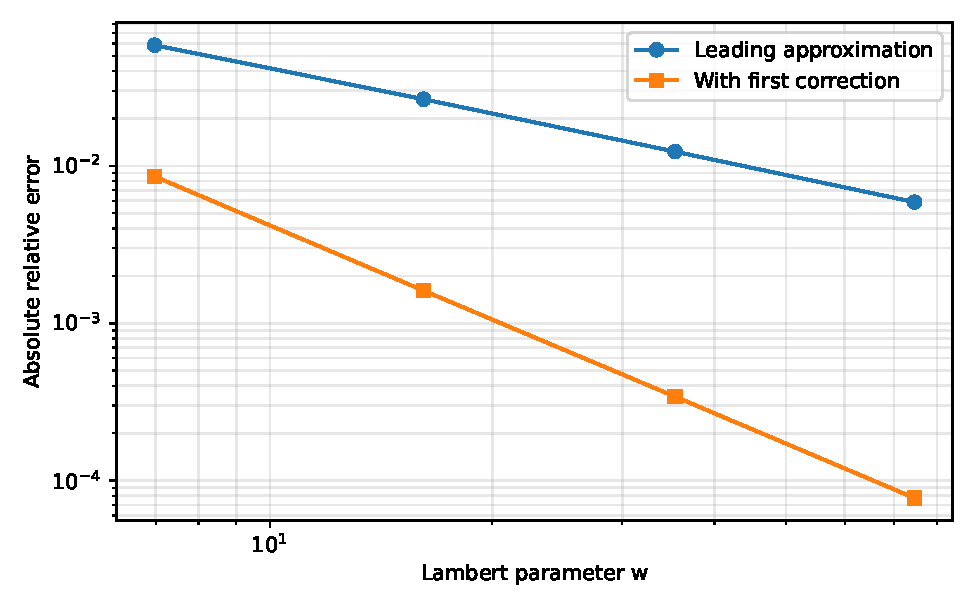
\includegraphics[width=0.87\textwidth]{saddle_errors.pdf}
\caption{Absolute relative errors for the data in Table~\ref{tab:saddle}.
The first correction improves the observed error from the scale \(1/w\)
to the scale \(1/w^2\), as predicted by the theorem. The graph is a numerical
check, not a uniform error bound.}
\label{fig:saddle}
\end{figure}

\subsection{The diagonal boundary layer}
For \(z=q=\e^{-t}\), direct logarithmic-product evaluation gives
Table~\ref{tab:boundary}. The signs of the errors need not be monotone; the
statement is a superalgebraic bound, not monotone convergence of the error.

\begin{table}[htbp]
\centering
\caption{The joint endpoint \(\Phi_q(q)\to1/\sqrt2\). Values are rounded;
the full data are in \texttt{boundary\_layer.csv}.}
\label{tab:boundary}
\begin{tabular}{@{}rrr@{}}
\toprule
\(t\)&\(\Phi_{\e^{-t}}(\e^{-t})\)&Error from \(1/\sqrt2\)\\
\midrule
1&0.758123053523105&\(5.1016\cdot10^{-2}\)\\
0.5&0.710249881663610&\(3.1431\cdot10^{-3}\)\\
0.25&0.706267615662706&\(-8.3917\cdot10^{-4}\)\\
0.125&0.707016842592727&\(-8.9939\cdot10^{-5}\)\\
0.0625&0.707106345877474&\(-4.3531\cdot10^{-7}\)\\
\bottomrule
\end{tabular}
\end{table}

\subsection{How to reproduce the archive}
The source is self-contained apart from the included vector figure. Run
\texttt{latexmk -pdf thue\_morse\_new\_directions.tex}, or run
\texttt{pdflatex} three times. The verification program requires Python 3.10
or later, \texttt{mpmath}, and \texttt{sympy}. Adding \texttt{--plots} also
uses \texttt{matplotlib} and regenerates the figure. Run
\texttt{python verify.py --plots} from the article directory. The program writes
its JSON summary and CSV tables beside itself.

The exact checks and floating-point checks are separated in the output. A
failed assertion stops the computation rather than silently producing a
success report. The numerical routines are intended for the explicitly stated
real parameter ranges; they are not implementations of analytic continuation
or a general complex saddle solver.

\section{Further deductions, limitations, and research directions}
\label{sec:frontiers}

\subsection{A unifying finite--infinite correspondence}
There are three distinct forms of compression in the proved results.
In the correlation problem, all interactions with a dyadic boundary are
compressed into the integer \(D(\bm h)\). In the nonlinear moment problem,
all Boolean cancellations are compressed into the covering condition
\(\bigcup\CCov=V\). In the product problem, the exact dyadic scaling is
compressed into the periodic amplitude \(\Psi\), while the continuous part
is handled by one saddle.

The comparison is structural, not an assertion that the three formulas are
special cases of a single theorem already proved here. Their common feature
is that cancellation is dealt with \emph{before} taking the asymptotic limit.
Doing the reverse can lose the boundary term, misidentify the first surviving
moment, or retain the wrong index in an infinite sum.

\subsection{Classifying vanishing boundary functionals}
\begin{question}
Which tuples \(\bm h\), modulo translations and deletion of repeated pairs,
satisfy \(D(\bm h)=0\)? Can their binary structure be characterized without
explicitly summing \eqref{eq:defect}?
\end{question}

For even order, \(D=0\) means every sufficiently large dyadic cyclic and
noncyclic sum equals its mean times the block length exactly. For odd order,
it means every sufficiently large aligned dyadic block sum is zero. This is
a finite classification problem with a precise observable consequence.
The pair recurrence \eqref{eq:Drec} provides a starting model, but the
higher-order combinatorics of the threshold parities \(b_t\) are richer.
No classification is claimed in this article.

\subsection{Designed nonlinear cancellation beyond a hafnian}
\begin{question}
For a prescribed sparse interaction graph, what is the largest possible
vanishing order of \(Z_x(t)\) among nontrivial signed quadratic weights,
subject to chosen normalization constraints on the linear part?
\end{question}

The positive-weight answer is determined by the minimum cover. Signed weights
allow algebraic cancellation among minimum covers, so the problem becomes a
finite polynomial system built from \eqref{eq:allmoments}. Useful constraints
would exclude degenerate choices that make \(x\) independent of a bit and
force \(Z_x\equiv0\). Requiring the coordinate map to be injective on the
Boolean cube is another natural way to rule out trivial pairwise coincidences.
The article supplies the equations but does not assert an optimal solution.

\subsection{Uniform matching of the two analytic regimes}
The fixed-\(z\) saddle corresponds to \(\beta=-\log z\) bounded away from zero,
while the boundary layer has \(\beta=\gamma t\). The intermediate regime
\(t\ll\beta\ll1\) should connect the large-\(\gamma\) asymptotics of
\(\mathcal H(\gamma)\) with the moving discrete saddle. A rigorous uniform
formula would need to control the relation between saddle width and mesh
size throughout that transition. Theorems~\ref{thm:saddle} and
\ref{thm:boundarylayer} establish the two endpoints but do not prove the full
uniform bridge.

\begin{question}
Can one construct a single asymptotic approximation, with an explicit
uniform remainder, valid when \(\beta/t\to\infty\) while \(\beta\to0\),
and matching both \eqref{eq:fullsaddle} and \eqref{eq:boundaryF}?
\end{question}

This is a concrete continuation problem rather than a request to speculate
about a nonexistent singularity. The exact positive representation
\eqref{eq:F} and the amplitude identity \eqref{eq:Afactor} remain valid
throughout the real parameter region and provide the required starting point.

\subsection{Beyond-all-orders corrections and complex parameters}
The saddle theorem suppresses lattice effects beyond every algebraic order
in \(1/w\). The boundary-layer theorem suppresses all Euler summation powers
of \(t\). Identifying the leading remaining corrections would require more
than extending the coefficient list: one must study the analytic continuation
of the amplitude and the relevant complex saddles or Fourier modes.
That problem is a natural transseries extension, but it is not solved by the
present all-order Poincar\'e expansion. Similarly, \(|z|=1\) is a boundary of
the absolute convergence arguments, and root-of-unity specialization requires
a fresh proof.

\subsection{Possible formalization targets}
The finite correlation and covering theorems have a relatively direct route
to formal proof: finite sums, bit decompositions, parity, and Boolean monomial
identities suffice. An initial formalization could isolate
\eqref{eq:blockfactor}, \eqref{eq:Vm}, and \eqref{eq:cover}, then derive the
remaining finite identities as corollaries. Such a project should use the
actual theorem names and conventions of the current repository after a
separate code audit; none are invented here.

The analytic results require additional infrastructure for infinite products,
termwise differentiation, dominated convergence, and uniform saddle estimates.
They should not be marked formalized merely because their numerical checks
pass. The supplied Python code is reproducibility material, not a proof
assistant certificate.

\section{Conclusion}
Three extensions of the Thue--Morse calculus have been obtained with explicit
formulas and proofs. The correlation theory admits a finite boundary functional
that gives exact defects at every order, including an odd-order telescoping
law and endpoint formulas involving an alternating binary digit sum. Nonlinear
Prouhet sums admit an exact hypergraph-cover expansion, making graph matchings
and hafnians the first surviving moment data of quadratic deformations. The
automatic geometric product \(\Phi_q(z)\) exhibits smooth flatness, a periodic
Lambert-\(W\) saddle law to every algebraic order, and a joint endpoint profile
that recovers classical paired Thue--Morse products with superalgebraically
small errors.

The results are concrete enough to test, extend, and formalize. Their historical
novelty remains a separate question from their mathematical validity: the
proofs establish the formulas, while the source audit provides a bounded,
explicitly stated comparison with existing work.

\appendix
\section{Coefficient generation without hidden recurrences}
\label{app:coefficients}

For a requested saddle order \(n\), formula \eqref{eq:cn} is a finite weighted
partition sum. An implementation can loop over \(k_j\) with
\(0\le k_j\le\lfloor2n/(j-2)\rfloor\), discard assignments for which
\(\sum(j-2)k_j>2n\), and set
\(\ell=2n-\sum(j-2)k_j\). This directly generates the coefficient in the
formal symbols \(A_0,\ldots,A_{2n}\). The program's recursive enumeration is
only a traversal of this finite index set; the mathematical coefficient formula
does not depend on previously computed coefficients.

The derivatives \(A_j\) can themselves be expressed as finite combinations of
\(\Psi^{(r)}(\theta)\). Let \(s=\log y\) and
\[
 B_\theta(s)=\e^{-s^2/(2a)}\Psi(\theta-s/a).
\]
Since \(\dd/\dd y=\e^{-s}\dd/\dd s\), induction gives
\begin{equation}
 \mathcal A_\theta^{(\ell)}(1)
 =\left.\left(\prod_{j=0}^{\ell-1}(D_s-j)\right)
                            B_\theta(s)\right|_{s=0},
 \qquad D_s=\frac{\dd}{\dd s}.
 \label{eq:Aoperator}
\end{equation}
For \(\ell=0\), the empty operator product is the identity. To prove the
formula, write
\(\dd^\ell/\dd y^\ell=\e^{-\ell s}\prod_{j=0}^{\ell-1}(D_s-j)\)
and differentiate once more; the derivative of \(\e^{-\ell s}\) introduces
the next factor \(D_s-\ell\).

If \(s(\ell,j)\) denotes the signed Stirling coefficient defined by
\(u(u-1)\cdots(u-\ell+1)=\sum_js(\ell,j)u^j\), then
\begin{equation}
 \mathcal A_\theta^{(\ell)}(1)
 =\sum_{j=0}^{\ell}s(\ell,j)
   \sum_{h=0}^{\lfloor j/2\rfloor}
       \frac{j!}{h!(j-2h)!}
       \left(-\frac1{2a}\right)^h
       \left(-\frac1a\right)^{j-2h}
       \Psi^{(j-2h)}(\theta).
 \label{eq:Astirling}
\end{equation}
Indeed, expand the Gaussian factor in even powers of \(s\), expand the
translated \(\Psi\) by its finite derivative coefficient, and extract the
\(j\)-th derivative at zero. Substituting \eqref{eq:Astirling} into
\eqref{eq:cn} produces a fully explicit finite formula for each saddle
coefficient in the derivatives of the periodic function.

\section{Notation and normalization reference}
\begin{longtable}{@{}p{0.23\textwidth}p{0.72\textwidth}@{}}
\toprule
Symbol&Meaning\\
\midrule
\endhead
\(\eps_n\)&The sign \((-1)^{s_2(n)}\), with \(\eps_0=1\).\\[2mm]
\(E(z)\)&The ordinary generating function \(\sum_{n\ge0}\eps_nz^n\).\\[2mm]
\(\bm h,H,p\)&A shift tuple with minimum zero, its maximum, and its length.\\[2mm]
\(D(\bm h)\)&The integer boundary functional in \eqref{eq:defect}.\\[2mm]
\(S_m,R_m\)&Noncyclic and cyclic sums over a block of length \(2^m\).\\[2mm]
\(\sigma(Q)\)&The alternating binary digit sum, not the ordinary digit sum.\\[2mm]
\(Z_x(t)\)&The signed exponential sum on a nonlinearly positioned Boolean cube.\\[2mm]
\(\HH,\tau\)&The family of nonempty monomial supports and its minimum cover size.\\[2mm]
\(\Haf(J)\)&The sum of products over perfect matchings; no determinant signs.\\[2mm]
\(\MM_G\)&The weighted matching polynomial, including unmatched singleton weights.\\[2mm]
\(\Phi_q(z)\)&The geometric product \(\prod_{j\ge0}(1-zq^j)^{\eps_j}\).\\[2mm]
\(A(x)\)&The positive product \(E(\e^{-x})\).\\[2mm]
\(Q(x)\)&The Laplace transform of \(\sum_{k\ge1}2^{-k}U_k\), with \(U_k\) uniform on \([0,1]\).\\[2mm]
\(\Psi(v)\)&The positive one-periodic function in \eqref{eq:Psidef}.\\[2mm]
\(F(t,z)\)&The positive logarithmic deviation \(-\log\Phi_{\e^{-t}}(z)\) for real positive \(z\).\\[2mm]
\(a,\beta,L\)&Respectively \(\log2\), \(-\log z\), and \(\log(1/t)\).\\[2mm]
\(w,r_*,\theta\)&The Lambert parameter, saddle location, and periodic phase in \eqref{eq:saddleparams}.\\[2mm]
\(P(t,z),c_n\)&The saddle prefactor and its periodic coefficient functions.\\[2mm]
\(\mathcal H,\mathcal P\)&The joint-endpoint integral and its exponential, distinct from the saddle prefactor \(P(t,z)\).\\
\bottomrule
\end{longtable}

\clearpage
\begin{thebibliography}{10}
\raggedright
\addcontentsline{toc}{section}{References}
\bibitem{atlas}
Vladimir Reshetnikov's ProveIt repository,
\emph{The Thue--Morse Sequence: Formula Atlas and Fabius--Rvachev Frontier Results},
consolidated \LaTeX\ source in
\nolinkurl{Analysis/FabiusFunction/docs/semi-formalized-research-frontiers/drafts/thue-morse/Thue_Morse_Atlas_and_Frontiers}.
\href{https://github.com/VladimirReshetnikov/ProveIt/tree/main/Analysis/FabiusFunction/docs/semi-formalized-research-frontiers/drafts/thue-morse/Thue_Morse_Atlas_and_Frontiers}{GitHub source directory}.
Mutable \texttt{main} source accessed 4 September 2026.

\bibitem{ubiquitous}
Jean-Paul Allouche and Jeffrey Shallit,
\emph{The ubiquitous Prouhet--Thue--Morse sequence}.
Author-hosted survey,
\url{https://cs.uwaterloo.ca/~shallit/Papers/ubiq15.pdf}.

\bibitem{baakecoons}
Michael Baake and Michael Coons,
\emph{Correlations of the Thue--Morse sequence},
arXiv:2209.07102v2, 4 March 2023.
\url{https://arxiv.org/html/2209.07102v2}.

\bibitem{bolker}
Ethan D. Bolker, Carl Offner, Robert Richman, and Catalin Zara,
\emph{The Prouhet--Tarry--Escott problem and generalized Thue--Morse sequences},
Journal of Combinatorics \textbf{7} (2016), no.~1, 117--133.
\url{https://arxiv.org/abs/1304.6756}.

\bibitem{ars}
Jean-Paul Allouche, Samin Riasat, and Jeffrey Shallit,
\emph{More infinite products: Thue--Morse and the gamma function},
Ramanujan Journal \textbf{49} (2019), 115--128.
\url{https://arxiv.org/abs/1709.03398}.

\bibitem{li}
Yao-Qiang Li,
\emph{Infinite products related to generalized Thue--Morse sequences},
arXiv:2006.04187, 2020.
\url{https://arxiv.org/abs/2006.04187}.

\bibitem{fgd}
Philippe Flajolet, Xavier Gourdon, and Philippe Dumas,
\emph{Mellin transforms and asymptotics: Harmonic sums},
Theoretical Computer Science \textbf{144} (1995), 3--58.
\url{https://specfun.inria.fr/dumas/Publications/FlGoDu95.pdf}.

\bibitem{dlmf}
NIST Digital Library of Mathematical Functions,
\S4.13, \emph{Lambert \(W\)-function}.
\url{https://dlmf.nist.gov/4.13}. Accessed 4 September 2026.

\bibitem{cloitre}
Benoit Cloitre,
\emph{The Thue--Morse transform}, arXiv:2604.06243v2,
28 May 2026. Preprint screened for related Prouhet constructions.
\url{https://arxiv.org/abs/2604.06243}.
\end{thebibliography}
\end{document}
